\documentclass[a4paper]{article}

\usepackage[english]{babel}
\usepackage[utf8x]{inputenc}
\usepackage{amsmath}
\usepackage{graphicx}
\usepackage{xcolor}
\usepackage{listings}
\usepackage{hyperref}
\usepackage{amssymb}
\usepackage[square,sort,comma,numbers]{natbib}
\usepackage[colorinlistoftodos]{todonotes}
\bibliographystyle{ieeetr}

\lstdefinestyle{julia}{
  basicstyle=\scriptsize\ttfamily,
  breaklines=false,
  backgroundcolor=\color{gray!10},
}
\lstset{style=julia,
        emph={julia},
        emphstyle={\color{green}\bfseries}}


\title{A Research Proposal on Mathematically Rigorous and Computationally
Efficient Representations of Geometry}
\author{Steve Kelly}

\begin{document}
\maketitle

\begin{abstract}
Geometry is fundamental to the development of natural problem statements.
Opportunities exist in computational geometry to
add rigourous type descriptions and algorithmic relations that do not
sacrifice performance. This proposal will develop a foundational context
for such a research project.
\end{abstract}

\section{Introduction}

Geometry is one of the earliest academic studies in mathematics. Research is
constantly leading to new patterns and constructions. Many of these find
highly practical applications in engineering. In this paper we will seek to
study geometry by developing patterns that are sensible to computers and people.
To obtain sensiblile patterns we address two different audiences.
One is the computer which requires execution effiency. The other is people,
who require lucid representation of code.

This proposal will try to refine existing implementations of geometry for
computers and explore new procedures. As such, we will review the existing
systems, their applications, and areas for improvement. Later we will discuss
some of the areas for improvement in more detail, and establish a proposed
scope for the project going forward.

\section{The Julia Programming Language}

Programming languages are the grammar and syntax a computer presents to a user.
This project is fundamentally exploratory in nature and seeks to generate
understanding of geometric relationships. I will use Julia as a programming
language for exploration. In the following sections I hope to develop some
rationale for this choice, and give a brief introduction to the language
concepts that will help make computationally effective geometry representations
possible,

\subsection{History}
Julia is a programming language first released in early 2012 by a group of
developers from MIT. The language targets technical computing by providing a
dynamic type system with near-native code performance. This is accomplished by
using three concepts: a Just-In-Time (JIT) compiler to target the LLVM framework,
a multiple dispatch system, and code specialization.\cite{bezanson2012julia}
The syntactical style is similar to MATLAB and Python.
The language implementation and many libraries are available under the
permissive MIT license.\footnote{\url{http://opensource.org/licenses/MIT}}

Benchmarks have shown the language can consistently perform within a factor of
two of native C and FORTRAN code.\footnote{\url{http://julialang.org/benchmarks}}
This is enticing for a solid modeling application and for numerical analysis,
as the code abstraction can grow organically without performance penalty.
In fact, the authors of Julia call this balance a solution to the 
``two language problem". The problem is encountered when abstraction in a
high-level language will disproportionately affect performance unless
implemented in a low-level language. In the next sections we will compare
the expressability and performance to other languages.

\subsection{Comparisons}

Julia is a descendent of the Lisp family of programming languages.


\begin{figure}[h!]
  \centering
    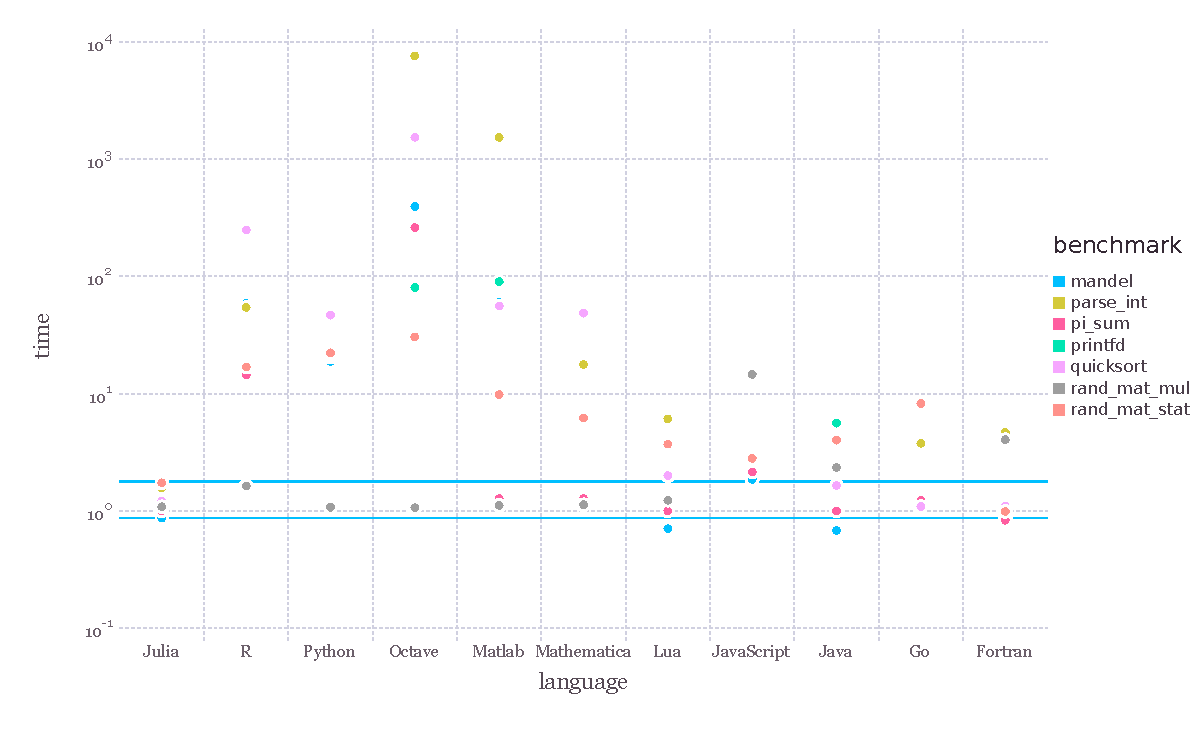
\includegraphics[width=1.0\textwidth]{img/juliabench.pdf}
  \caption{A comparison of programming languages and performance.}
  \label{fig:juliabench}
\end{figure}

\begin{figure}[h!]
  \centering
    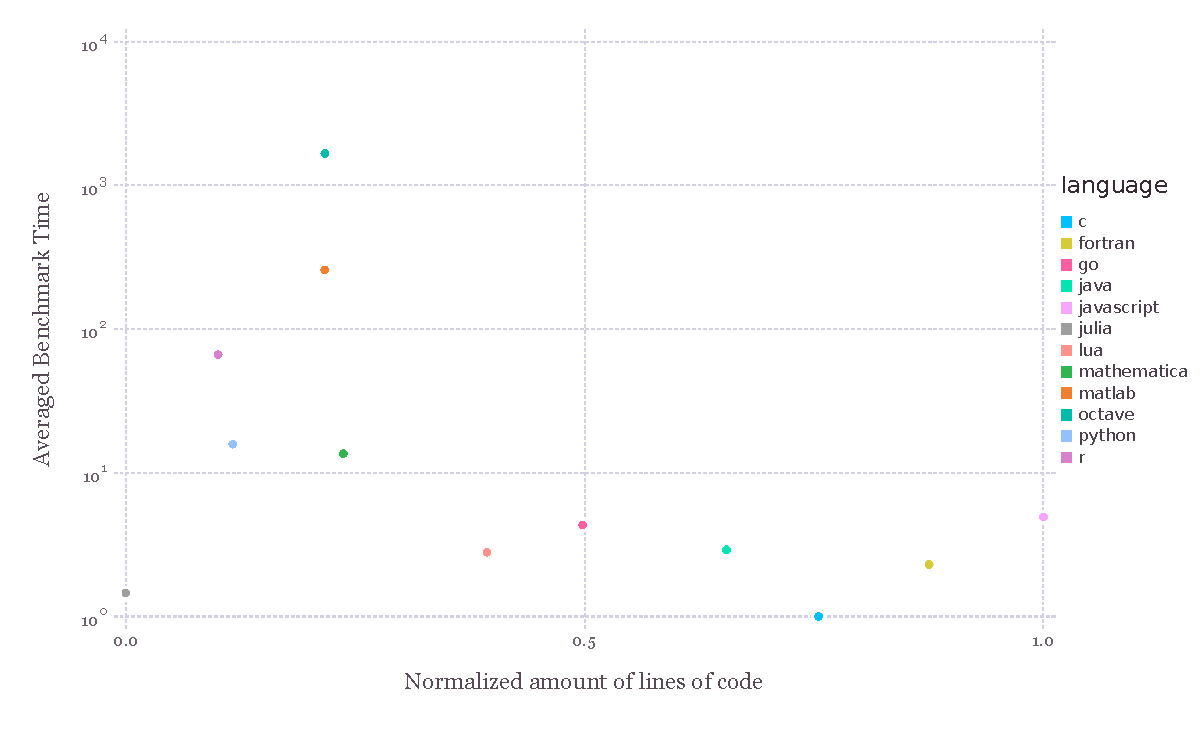
\includegraphics[width=1.0\textwidth]{img/expressability.pdf}
  \caption{The results in Figure \ref{fig:juliabench} normalized for code length.}
  \label{fig:juliaexpr}
\end{figure}


\begin{figure}[h!]
  \label{tab:types}
  \centering
    \caption{A comparison of functions, typing, and dispatch.}
    \begin{tabular}{ l | l l l}
    Language & Type system & Generic functions & Parametric types \\
    \hline
    Julia & dynamic & default & yes \\
    Common Lisp & dynamic & opt-in & yes (but no dispatch) \\
    Dylan & dynamic & default & partial (no dispatch) \\
    Fortress & static & default & yes \\
    \end{tabular}
\end{figure}


\subsection{Functions}
Julia is an experiment in language design. Much of the advancement
revolves around the representation of data and the execution of functions.
The language is optionally typed, which means function specialization on types
is inferred. See below:
\begin{lstlisting}
julia> increment(x) = x + 1
increment (generic function with 1 method)

julia> increment(1)
2

julia> increment(1.0)
2.0
\end{lstlisting}
the \texttt{increment} function was defined for any \texttt{x} value. When the
\texttt{1}, an
integer type was passed as an argument, an integer was returned. Likewise
when a floating point, \texttt{1.0} was passed, the floating point
\texttt{2.0} was returned.

Let's see what happens when we try a string:
\begin{lstlisting}
julia> increment("a")
ERROR: MethodError: `+` has no method matching +(::ASCIIString, ::Int64)
Closest candidates are:
  +(::Any, ::Any, ::Any, ::Any...)
  +(::Int64, ::Int64)
  +(::Complex{Bool}, ::Real)
  ...
 in increment at none:1
\end{lstlisting}

The problem is that the \texttt{+} function is not implemented between the
\texttt{ASCIIString} and \texttt{Int64} types.
We need to either implement a \texttt{+} function
which might be ambiguous, or specialize the function for \texttt{ASCIIString}.
A specific implementation is preferrable in this case:
\begin{lstlisting}
julia> function increment(x::ASCIIString)
           ASCIIString([increment(c) for c in x])
       end
increment (generic function with 2 methods)
\end{lstlisting}
The line \texttt{x::ASCIIString} is called a ``type annotation" and
states that \texttt{x} must be a subtype
of \texttt{ASCIIString}. This allows one to control dispatch of functions,
since Julia will default to the \emph{most specific implementation}.
Since\texttt{ASCIIString} is a series of 8 bit characters, we can iterate over the
string and increment each character individually. The \texttt{[]} indicates we are
constructing an array of characters to pass to be passed to the \texttt{ASCIIString}
type constructor. Now we see our example works:
\begin{lstlisting}
julia> increment("abc")
"bcd"
\end{lstlisting}

What was demonstrated here is the concepts of specialization and multiple
dispatch, both are highly coupled topics.
Each function call in Julia is specialized for types if possible.
This means the author only has to write a few sufficently abstract
implementations of functions. If special cases occur multiple functions
with different arity or type signatures can be implmented. Explicitly
this is called multiple dispatch. In practice by the user this looks like
abstracted or generic code.
To the computer, this means choosing the most specific, and
thus performant method. Let's go back to the integer and floating point
example. Below is the LLVM assembly generated for each method:
\begin{lstlisting}
julia> @code_llvm increment(1)

define i64 @julia_increment_21458(i64) { // <return type> <function name>(<arg type>)
top:
  %1 = add i64 %0, 1
  ret i64 %1 // return <return type> <return id>
}

julia> @code_llvm increment(1.0)

define double @julia_increment_21466(double) {
top:
  %1 = fadd double %0, 1.000000e+00
  ret double %1
}
\end{lstlisting}

The only real similarity is the line count. Note I have annotated the LLVM code
so this is understandable. Each one of these functions are generated by the
Julia compiler at run time. The REPL (Read-Eval-Print-Loop) allows interactive
evaluation of Julia code. It is highly useful for exploration and testing of
ideas.

Many of the concepts used for performance also serve as methods for
expressability. In this case, multiple dispatch used by the compiler for
specialization of functions reveals it self as a way for the user to
specialize over many types.
Revealing the role in which this paradigm allows Julia to achieve high
performance is a matter to be developed in further sections.

\subsection{Types}

\subsubsection{Mutability and data packing}
Types and immutables are containers of data. The primary difference between
the two is the notion of "mutability". Types are mutabile, immutables are 
immutable. What does this mean? Let's break something first:
\begin{lstlisting}
julia> type FooIsMutable
           a
       end

julia> f = FooIsMutable(1)
FooIsMutable(1)

julia> f.a
1

julia> f.a = 2
2

julia> f.a
2

julia> immutable FooIsImmutable
           a
       end

julia> f = FooIsImmutable(1)
FooIsImmutable(1)

julia> f.a
1

julia> f.a = 2
ERROR: type FooIsImmutable is immutable
\end{lstlisting}

What just happened demonstrates the contract defined by mutability. Mutable
objects, which is an instance of a type (i.e. \texttt{f}), can have their fields
(i.e. \texttt{a}) changed. Immutables cannot. The immutable contract helps develop
a notion of functional purity. To the user this means immutables are defined
by their values. Practically this can be of great benefit to
the compiler. For example:
\begin{lstlisting}
julia> a = (1,2,3)
(1,2,3)

julia> b = typeof(a)
Tuple{Int64,Int64,Int64}

julia> isbits(b)
true

julia> a = ([1],[2],[3])
([1],[2],[3])

julia> b = typeof(a)
Tuple{Array{Int64,1},Array{Int64,1},Array{Int64,1}}

julia> isbits(b)
false
\end{lstlisting}

\texttt{isbits} ask the question ``will this type be tightly packed in memory"? A
\texttt{Tuple} is a fixed-length set of linear, ordered, data. It has syntax for
construction with \texttt{()}. In computations we want our data be close together
for fast access. In modern times we call such data "cache friendly", or
"cache localized". Immutability helps us achieve this. Let's look that the
types inside the 3-tuples and see their \texttt{isbits} status:
\begin{lstlisting}
julia> isbits(Array{Int64,1})
false

julia> isbits(Int64)
true
\end{lstlisting}
Why is this the case? We see that \texttt{Int64} is bits, because it is literally
64 bits. In Julia a \texttt{bitstype} behaves similar to an immutable, and is identified
by value. \texttt{Array\{Int,64\}} is a mutable data type that can vary in size.
This means
the \texttt{Tuple} needs to store the arrays as references, in this case a
pointer. When iterating over a data set, such a ``pointer dereferences" (this is
jargon for accessing the data in memory pointed to by a pointer), can be costly.
Modern CPUs accell when data is linearly packed and pointer-free. The
data can be brought into the CPU's memory cache once and computed without
shuffling between cache and RAM.

\subsubsection{Parameters}


\subsection{Example}


\section{Solid Modeling Paradigms}

The expression of solid bodies is fundamental in the development of any
natural problem statement. For example, in diffusion we model the transfer of
energy throughout a domain. An engineer might define such a domain with a
model, say of an injection molding nozzle. Such a domain is difficult to
describe in terms of a functional boundary, so the engineer might prefer
a boundary representation.

In addition to being fundamental to natural studies, solid modelling is growing
in popularity due to low-cost digital manufactuing tools reaching the market.
Most popularly there have been 3D printers popping up in nearly every educational
insitiution over the past 3 years. In addition CNC routing, and laser cutting
enable people to go quickly from design to fabrication.


The development of modern
computational tools for solid modeling have vastly different paradigms. In
the next few sections we will layout the mathematical and computational
primciples of these paradigms.

\subsection{Implicit Functional Representation}

Functional representation in computation centers around a signed, real-value
function where the boundary is defined as $f(...) = 0$.
In $\mathbb{R}3$ this looks like $f(x,y,z) = 0$. For modelling purposes we must add the
additional constraint that the function evaluates to a negative inside the
boundary. Further more the magnitude of the return value must correspond to
the minimum distance between the point and the boundary. \cite{Olah_2011}


\subsubsection{Distance Fields}

\cite{OpenVDB}

\paragraph{Mesh Construction}
\cite{Tzur}

\paragraph{Visualization}
\cite{Tupper_2001}

\subsection{Mesh}

\cite{Bischoff_Botsch_Steinberg_Bischoff_Kobbelt_Aachen_2002}

\subsection{Boundary Rep}
Boundary Representation (B-Rep) has been the dominant modelling paradigm
for engineering since the 1970's.
It relies primarily on the manipulation and representation of
edges, vertices, and faces to build a model.
The primary mechanism for the representation is a "feature tree".
While B-Rep is intuitive for users of a graphical environment,
it is unwieldy as a textual and functional representation.
This methods is natural for engineers and designers, but sacrifices
parametric design. In addition, B-Rep requires the use of a geometry kernel
to handle the interpretation of constraints and geometric construction. \cite{stroud2006boundary}

Geometry kernels often decouple functional representations from a user's design
hierarchy which complicates numerical analysis.\cite{lee2005cad}
This middle step of Computer Aided Engineering (CAE) is known as pre-processing.
For example in the Finite Element Analysis (FEA) process the requires
establishing proper aspect ratio, area, and connectivity of nodes. Research has shown that functional representations can simplify or eliminate these steps and algorithms.





\subsection{CSG}

In addition, designers targeting parametric design have turned to the methods
of Constructive Solid Geometry (CSG), which works using manipulation of
geometric primitives (half-spaces) as a level of abstraction.
This enables parametric solids to be represented using operations and
relations on primitive solids. CSG has been growing in popularity due
to programs such as OpenSCAD\footnote{\url{http://www.openscad.org}},
CoffeeSCAD\footnote{\url{http://coffeescad.net/}},
POVRay\footnote{\url{http://www.povray.org/}}
and Thingiverse Customizer\footnote{\url{http://www.thingiverse.com}}.
These programs are particularly popular for collaboration
in conjunction with version control systems such as Git.

\begin{figure}[h!]
  \centering
    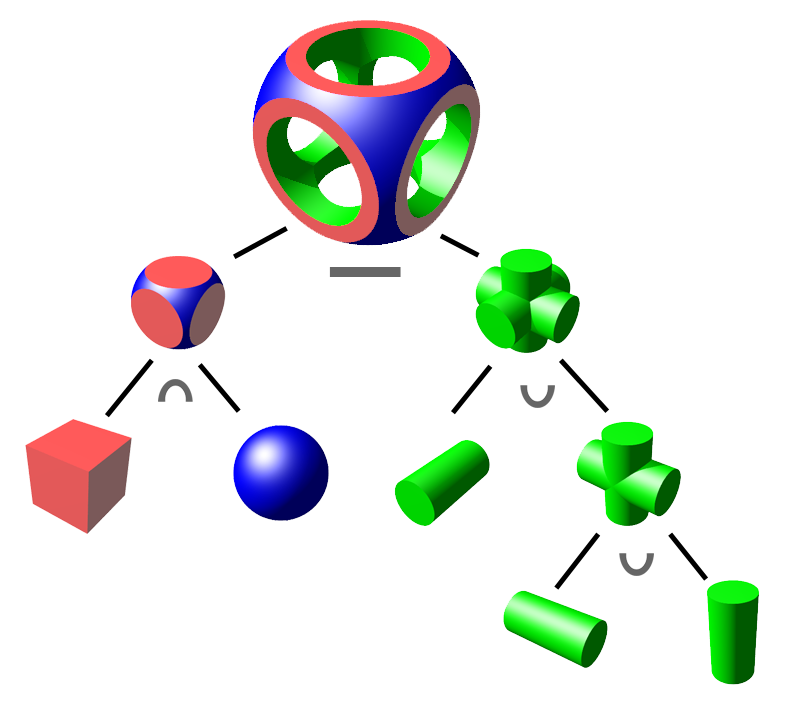
\includegraphics[width=0.75\textwidth]{img/csg_tree.png}
  \caption{An illustration of a CSG tree.}
\end{figure}


\subsection{Graphs}

Laplacian Contractions!!!


\paragraph{Functional Reactive Programming}

\section{Representation for Simulation Methods}


\subsubsection{Linear Algebraic Representation}
\cite{DiCarlo_Paoluzzi_Shapiro_2014}

\section{Exploration}

\subsection{Rigorous Definitions of Geometry}

GeometryTypes.jl is a package for Julia that provides geometric strutures and
relations. It was started early 2015 as the integration of Meshes.jl,
ImmutableArrays.jl, HyperRectangles.jl, and FixedSizeArrays.jl. This package
was able to resolve the relations between so geometric structures for
computational agorithms and fast visualization the GPU. With the
release of Julia version 0.4 is became possible to build the appropriate
abstractions. For example ImmutableArrays represented a 3 dimensional
vector with the concrete type `Vector3{Int64}`. FixedSizeArrays introduced
the dimensionality as a parameter as `Vector{3,Int64}`. This means the notion
of a fixed length vector can be abstracted over arbitrary dimensionality.

\subsubsection{Numerical Robustness}


\cite{Gappa}

\subsubsection{Simplices}

Recently a `Simplex` type was added to `GeometryTypes`. A `Simplex` is defined
as the minimum convex set containing the specified points. The initial
prototype
%https://en.wikipedia.org/wiki/Simplicial_complex

\subsubsection{Distance Fields}

Lagrangian and Eulerian specification of the flow field



\subsection{Automatic Differentiation}

\subsubsection{Dual Numbers}
\begin{lstlisting}
julia> using DualNumbers

julia> f(x) = 2x+1
f (generic function with 1 method)

julia> f(Dual(1,1))
3 + 2du
\end{lstlisting}


\subsubsection{Rvachev Functions}


In the 1960's Vladimir Rvachev produced a method for handling the "inverse
problem of analytic geometry". His theory consists of functions which provide a
link between logical and set operations in geometric modeling and analytic
geometry.\cite{shapiro1991theory} I believe the following anecdote helps
elucidate the theory. While attempting to solve boundary value problems,
Rvachev formulated an equation of a square as
\begin{equation*}
a^2 + b^2 − x^2 − y^2 + \sqrt[]{( a^2 − x^2 )^2 +( b^2 − y^2 )^2} =0
\end{equation*}

Implicitly, the sides of a square can be defined as $x= +/- a$ and $y= +/- b$.
The union of these two is a square. By reducing the formulation of the square
we can generalize an expression for the union between two functions.
\begin{equation*}
\cup : f_1 + f_2 + \sqrt[]{f_1^2 +f_2^2} =0
\end{equation*}

Likewise we can see that intersections and negations can be formed for logical
completion.
\begin{equation*}
\cap : f_1 + f_2 - \sqrt[]{f_1^2 +f_2^2} =0 \\
\end{equation*}
\begin{equation*}
\neg : -f_1
\end{equation*}

These formulations can be modified for $C^m$ continuity for any $m$.
\cite{shapiro2007semi} In addition Pasko, et. al. have shown that Rvachev
functions can serve to replace a geometry kernel by creating logical
predicates. \cite{pasko1995function} Their research also establishes the
grounds for user interfaces and environment description. For this work a
practical implementation will most likely leverage their insights.
Rvachev and Shapiro have also shown that using the POLE-PLAST and SAGE
systems a user can generate complex semi-analytic geometry
as well.\cite{rvachev2000completeness} 
\subsection{Numerical Analysis}
While a functional representation for geometry is mathematically enticing on
its own, the power it gives for numerical analysis might be its greatest
virtue. Numerical analysis justified the initial investigation by Rvachev
early on. A boundary value problem on a R-Function-predicate domain allows
for analysis without construction of a discrete mesh.\cite{rvachev2000completeness}

One of the most general expositions in the English language of R-Functions
applied to BVPs is
Vadim Shapiro's``Semi-Analytic Geometry with R-Functions". \cite{shapiro2007semi}
Unfortunately, no monographs about R-Functions exist in the English literature.
Most literature is in Russian, however many articles presenting applied
problems using the R-Function Method. \cite{voron2010} This is the topic
of this project I stand to gain the most insight.


\subsection{Geometry in Path Planning}

\subsubsection{Mesh Slicing}


\section{Conclusion}


\bibliography{references}

\end{document}

